\chapter{Huấn luyện, lựa chọn cấu hình và hiệu chỉnh}\label{chap:training}
\FloatBarrier
\section{Giao thức lựa chọn và thông số thực nghiệm}
Các mô hình dùng cùng tập dữ liệu và phép chia, nhưng có mục tiêu tối ưu, trọng số và ngân sách lựa chọn khác nhau. Tất cả cấu hình được đánh giá trên test được chọn bằng validation. Từ vựng/IDF, từ vựng chuỗi và trọng số lớp chỉ học từ train; test không dùng chọn cấu hình, epoch, temperature hoặc hệ số quyết định.
\begin{table}[htbp]\centering\small\caption{Thiết lập lựa chọn và thiết bị; cấu hình biểu diễn chi tiết ở chương~\ref{chap:model}.}\label{tab:training_protocol}
\begin{tabularx}{\linewidth}{lXXl}\toprule Mô hình & Ngân sách lựa chọn & Tiêu chí và tối ưu & Thiết bị\\\midrule
SVM & 12 cấu hình; chỉ học từ tập huấn luyện TF--IDF & Hội tụ squared hinge; Macro-F1 validation & CPU, 4 luồng\\
LR & 12 cấu hình; chỉ học từ tập huấn luyện TF--IDF & Hội tụ mất mát logarit; Macro-F1 validation & CPU, 4 luồng\\
BiLSTM & 3 cấu hình; tối đa 10 epoch/lượt & AdamW; bản lưu mô hình theo Macro-F1 & RTX A3000\\
PhoBERT & Cấu hình cố định; tối đa 7 epoch & AdamW; bản lưu mô hình theo Macro-F1 & RTX A3000\\\bottomrule
\end{tabularx}\end{table}
Validation còn được dùng ước lượng tham số hiệu chỉnh nên kết quả có phụ thuộc vào tập này; một tập hiệu chỉnh xác suất riêng là hướng kiểm tra thêm. Seed 42 khóa phép chia trong bản dữ liệu, chưa bảo đảm phép tính GPU giống bit giữa thiết bị/phiên bản. Ngân sách tìm cấu hình khác nhau cần được giữ khi diễn giải đánh đổi, thay vì coi đây là một phép thay kiến trúc có kiểm soát mọi yếu tố.

\FloatBarrier
\section{Huấn luyện SVM/LR và BiLSTM}
\section{Huấn luyện và lựa chọn hai mô hình tuyến tính}
SVM và LR mỗi model khảo sát 12 cấu hình từ hai profile unigram/unigram--bigram, ba giá trị $C\in\{0,5;1,5;3,0\}$ và hai chính sách trọng số lớp uniform/balanced. Các profile được fit độc lập chỉ trên train; classifier dùng cùng ma trận của profile tương ứng. Với balanced, trọng số $w_c=N_{train}/(20n_c)$ dựa trên phân bố train, không cân bằng lại validation/test.

Validation chọn cấu hình bằng Macro-F1, tiếp đến Weighted-F1 và Accuracy khi bằng nhau. Mỗi cấu hình phải đạt hội tụ trước khi đủ điều kiện được chọn. Output xác nhận cả 12 cấu hình SVM và 12 cấu hình LR hội tụ; cấu hình được giữ là hai cấu hình trong bảng~\ref{tab:linear_config}. Không lấy cấu hình tốt nhất theo test và không refit thêm validation vào train sau lựa chọn. Chi phí tìm cấu hình được ghi riêng với thời gian fit classifier đã chọn.

\section{Huấn luyện BiLSTM và chọn checkpoint}
\label{sec:lstm_training}
Ba cấu hình khảo sát kết hợp Head--Tail 256/512 từ với số mũ trọng số lớp 0,5/1,0; các thành phần kiến trúc còn lại giữ như mục~\ref{sec:bilstm}. Báo cáo phân tích cấu hình được chọn: 512 từ, embedding 200, hidden 128 mỗi hướng, một layer, dropout 0,35 và $\alpha=0,5$. Trọng số được chuẩn hóa theo trung bình có trọng số của train:
\begin{equation}
\widetilde w_c=\left(\frac{N_{train}}{20n_c}\right)^{\alpha},\qquad
w_c=\frac{\widetilde w_c}{\sum_j(n_j/N_{train})\widetilde w_j}.
\end{equation}
Nông thôn mới có trọng số 3,3510 trong cấu hình này, khác 10,3226 của PhoBERT. Loss của batch là tổng cross-entropy có trọng số chia tổng trọng số các nhãn trong batch. Loss epoch được cộng từ các tử số và mẫu số, không lấy trung bình không trọng số giữa batch đầy và batch cuối.

\begin{table}[H]\centering\small\caption{Tối ưu BiLSTM của cấu hình được chọn.}\label{tab:bilstm_training}
\begin{tabular}{lr}\toprule Thiết lập & Giá trị\\\midrule
Optimizer & AdamW\\
Learning rate ban đầu / tối thiểu & $10^{-3}$ / $10^{-5}$\\
Weight decay / gradient clip & $10^{-4}$ / 1,0\\
Batch train / validation và test & 64 / 128\\
Epoch tối đa / epoch đã chạy & 10 / 10\\
Checkpoint chọn & Epoch 10\\
Early stopping patience / min delta & 2 / 0,001\\
ReduceLROnPlateau factor / patience & 0,5 / 0\\
GPU / precision & RTX A3000 12 GB / BF16\\\bottomrule
\end{tabular}\end{table}

AdamW cập nhật embedding, recurrent layer và classifier. AMP dùng BF16; gradient được clip về norm tối đa 1,0 trước bước optimizer. Scheduler theo Macro-F1 validation, giảm learning rate một nửa sau epoch không cải thiện đủ ngưỡng tuyệt đối 0,001. Batch giữ phân bố train thực tế qua shuffle; trọng số loss không tương đương oversampling lớp hiếm.

Checkpoint và early stopping có tiêu chí khác nhau: checkpoint giữ giá trị validation tốt nhất kể cả cải thiện nhỏ; bộ đếm dừng cần vượt mốc tốt trước đó ít nhất 0,001. Vì vậy, epoch 10 có Macro-F1 0,8449 cao nhất nhưng vẫn kích hoạt bộ đếm patience sau hai epoch không cải thiện đủ ngưỡng. Thực nghiệm đã chạy 10 epoch; không mô tả như được dừng trước giới hạn. Bảng và các đồ thị dưới đây thuộc duy nhất cấu hình được chọn, không nối lịch sử của ba cấu hình.
\DataTable{tables/lstm_epochs.tex}{Lịch sử 10 epoch của BiLSTM được chọn; loss có trọng số, checkpoint theo Macro-F1.}
Loss validation thấp nhất ở epoch 5 (0,4230), trong khi Macro-F1 cao nhất ở epoch 10 (0,8449). Loss train giảm từ 1,2428 xuống 0,2360; loss validation cuối là 0,4341. Chênh lệch này cảnh báo về mức phù hợp giữa train và validation, nhưng không đủ để quy mọi thay đổi F1 cho overfitting. Weighted loss, Macro-F1 và calibration đánh giá các tính chất khác nhau.
\ReportFigure{assets/baselines/lstm/training/train_loss.png}{Weighted cross-entropy train của BiLSTM qua 10 epoch, xuất riêng từ notebook.}
\ReportFigure{assets/baselines/lstm/training/validation_loss.png}{Loss validation của BiLSTM; cực tiểu loss không trùng checkpoint Macro-F1 tốt nhất.}
\ReportFigure{assets/baselines/lstm/training/validation_f1_macro.png}{Macro-F1 validation của BiLSTM; checkpoint được chọn ở epoch 10.}
\ReportFigure{assets/baselines/lstm/training/learning_rate.png}{Learning rate theo epoch của BiLSTM; giảm từ 0,001 đến 0,000125.}

\section{Hiệu chỉnh điểm số của các mô hình đối chứng}
SVM tạo margin, LR và BiLSTM tạo logits. Cả ba dùng $p(T)=\operatorname{softmax}(s/T)$, tìm $T>0$ bằng NLL trên validation và cố định trước đánh giá test. SVM dùng phép chuẩn hóa margin thành phân bố, không có xác suất sinh sẵn từ \texttt{LinearSVC}. Temperature dương giữ thứ tự score, nên Accuracy, precision, recall và F1 không thay đổi. Ba đối chứng không dùng hệ số điều chỉnh quyết định theo lớp như PhoBERT.

Validation phục vụ cả lựa chọn model lẫn fit temperature. Việc dùng lại validation có thể tăng phụ thuộc vào tập này; test vẫn không tham gia fit. Khoảng tin cậy trong notebook dùng bootstrap IID 500 lần trên test với model cố định. Nó mô tả biến thiên do mẫu đánh giá, không mô phỏng nhiều lần huấn luyện với seed khác nhau. So sánh ghép cặp ở chương~\ref{chap:comparison} giữ chung các mẫu bootstrap để đánh giá chênh lệch giữa model.

\section{Fine-tuning và hiệu chỉnh PhoBERT}
Các mục sau mô tả quy trình PhoBERT; trọng số, optimizer, lịch học và hệ số quyết định thuộc cấu hình riêng của mô hình. Phép chia và tiêu chí đánh giá thống nhất với ba đối chứng, còn cách biểu diễn và ngân sách tìm tham số khác nhau. Mọi kết luận về đóng góp riêng của Head--Tail, trọng số lớp hoặc pretraining cần một ablation tương ứng.




Điều kiện hội tụ của SVM/LR xác nhận optimizer đã đạt tiêu chí số của cấu hình, không chứng minh mô hình tối ưu về nhãn hay tổng quát hóa. Với LR, L-BFGS tối ưu mất mát logarit có điều chuẩn; với LinearSVC, mục tiêu squared hinge theo các bài toán một-chống-còn-lại. Cùng Macro-F1 validation để lựa chọn không làm hai mục tiêu train trở thành giống nhau. Số vòng tối ưu vì thế không so trực tiếp như số epoch của mạng nơ-ron.

Mỗi cấu hình ứng viên được học từ train trước khi đo trên validation. Không dùng test để loại cấu hình ứng viên hội tụ nhưng có điểm thấp, và không gộp train/validation rồi ước lượng lại một gói mô hình có điều kiện khác với gói mô hình đo test. Kết quả được báo cáo thuộc cấu hình đã chọn, còn chi phí tìm cấu hình tính toàn bộ ứng viên. Khoảng giữa thời gian huấn luyện cấu hình được chọn và tìm cấu hình phản ánh khác biệt giữa dùng lại một thiết lập và tìm ra thiết lập đó.

Với BiLSTM, loss train giảm chưa là tiêu chí nạp bản lưu mô hình cuối. Chọn bản lưu mô hình theo Macro-F1 và bộ đếm early stopping có ngưỡng cải thiện riêng, nên một epoch có thể tạo bản lưu mô hình tốt nhất dù không đặt lại bộ đếm dừng sớm. Cơ chế này giải thích vì sao lịch sử đủ 10 điểm và bản lưu được chọn ở epoch 10 cùng tồn tại; không cần suy một đợt train khác hoặc nối hai lịch sử.

\FloatBarrier
\section{Fine-tuning PhoBERT và diễn biến validation}
Mô hình khởi tạo từ \texttt{vinai/phobert-base-v2}; đầu phân loại 20 lớp được tạo cho tác vụ. Toàn bộ encoder và đầu phân loại được cập nhật qua lan truyền ngược, không giữ cố định bộ mã hóa nền. Train tensor có $139{,}975\times256$ vị trí; validation/test có $29{,}995\times256$. Input IDs, attention mask và nhãn giữ thứ tự, train shuffle batch còn các tập đánh giá giữ phân bố thực tế.

Với $n_c$ là số bài lớp $c$ trong train, PhoBERT dùng balanced weight:
\begin{equation}w_c=\frac{N_{train}}{20n_c},\qquad
\mathcal L_{\mathcal B}=\frac{-\sum_{i\in\mathcal B}w_{y_i}\log p_{i,y_i}}{\sum_{i\in\mathcal B}w_{y_i}}.\end{equation}
Không tăng thêm trọng số cho một chuyên mục bằng hệ số đặt thủ công. Nông thôn mới, Dân tộc thiểu số và miền núi, Kinh doanh có trọng số lần lượt 10.3226; 9.1847; 0.7908. Trọng số thay đổi mức đóng góp của lỗi, không bổ sung dữ liệu hoặc làm sạch nhãn; nếu lớp nhỏ có nhiễu, tăng mức phạt trong hàm mất mát có thể khuếch đại ảnh hưởng đó. Mất mát đánh giá có trọng số cũng khác NLL hiệu chỉnh xác suất không trọng số.

\begin{table}[htbp]\centering\small\caption{Cấu hình fine-tuning PhoBERT trên một RTX A3000 Laptop 12 GB.}
\begin{tabular}{lr}\toprule Thiết lập & Giá trị\\\midrule
Batch train / tích lũy gradient & 32 / 2\\
Effective batch / batch đánh giá & 64 / 64\\
Optimizer / weight decay & AdamW fused / 0.01\\
Learning rate cực đại / warmup & $2\times10^{-5}$ / 200 bước\\
Độ chính xác số / TF32 & BF16 / bật\\
Epoch tối đa / bản lưu được chọn & 7 / 7\\
Dừng sớm: số epoch chờ / mức cải thiện & 2 / 0.001\\
Evaluation và lưu bản lưu mô hình & Cuối mỗi epoch\\
Lưu lại tính toán gradient / biên dịch mô hình & Tắt / tắt\\\bottomrule
\end{tabular}\end{table}
AdamW tách weight decay khỏi cập nhật thích nghi \citep{adamw}. Scheduler warmup 200 bước rồi giảm theo tiến độ. Mỗi epoch có $\lceil139{,}975/32\rceil=4{,}375$ mini-batch, tạo 2,188 bước cập nhật sau tích lũy; bảy epoch có 15,316 bước. Batch cuối có thể nhỏ hơn effective batch 64, nên con số này là kích thước danh nghĩa.

Trainer chọn bằng Macro-F1 validation và nạp bản lưu mô hình tốt nhất ở cuối. Lần thực nghiệm chạy đủ bảy epoch; không mô tả như dừng sớm. Loss validation nhỏ nhất epoch 3 là 0.3548, trong khi bản lưu mô hình chọn epoch 7 có Macro-F1 khoảng 0.8723. Bảng~\ref{tab:pho_epochs} giữ mốc validation; test không dùng đổi tiêu chí sau khi xem kết quả.
\begin{table}[htbp]\centering\small\caption{Đánh giá cuối epoch trên validation PhoBERT.}\label{tab:pho_epochs}
\begin{tabular}{rrr}\toprule Epoch & Val loss & Val Macro-F1\\\midrule
1 & 0,4034 & 0,8343\\
2 & 0,3581 & 0,8538\\
3 & 0,3548 & 0,8597\\
4 & 0,3717 & 0,8660\\
5 & 0,4257 & 0,8718\\
6 & 0,4592 & 0,8708\\
7 & 0,4980 & 0,8723\\
\bottomrule\end{tabular}
\end{table}
\begin{figure}[tbp]\centering
\begin{subfigure}[t]{.48\textwidth}\centering
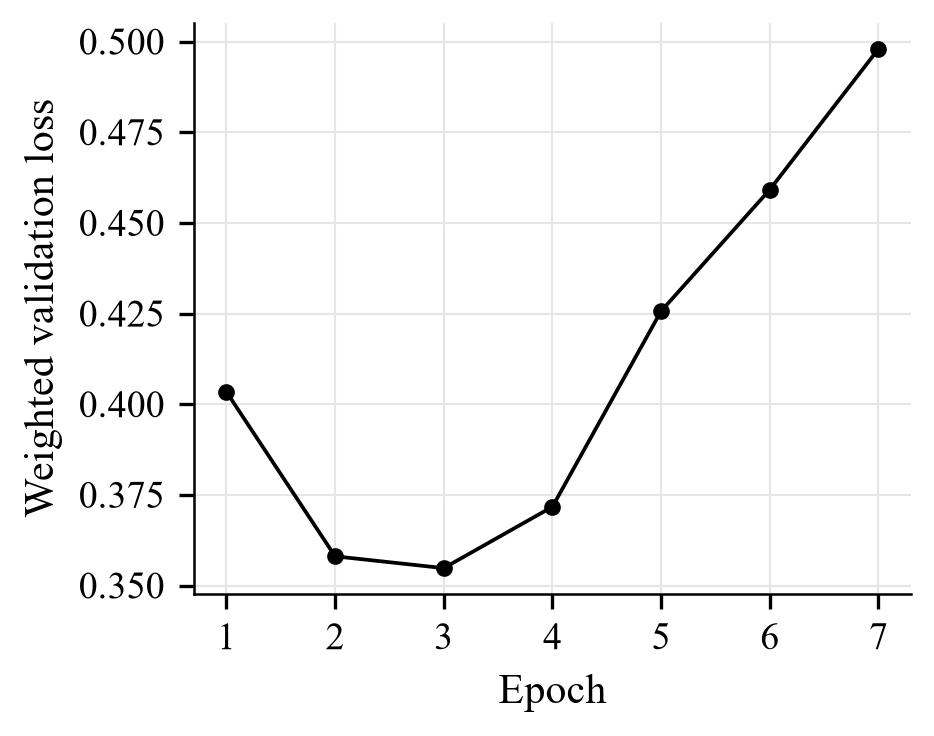
\includegraphics[width=\linewidth]{assets/compact/pho_val_loss.png}\caption{Mất mát trên tập xác thực có trọng số.}\end{subfigure}\hfill
\begin{subfigure}[t]{.48\textwidth}\centering
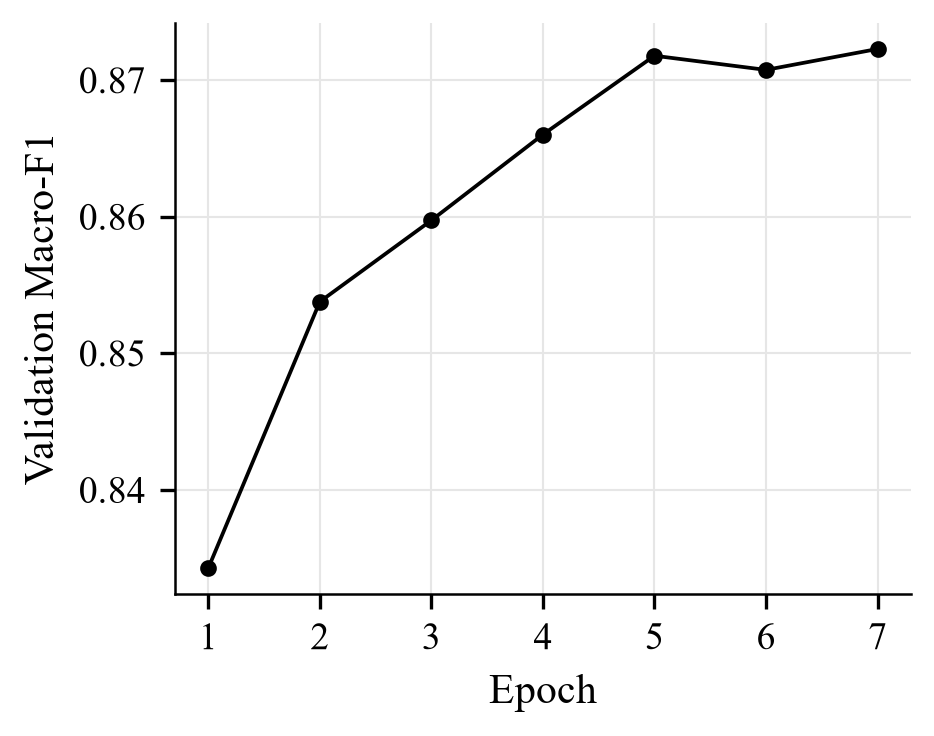
\includegraphics[width=\linewidth]{assets/compact/pho_val_f1.png}\caption{Macro-F1 trên tập xác thực.}\end{subfigure}
\caption{PhoBERT qua bảy epoch; lựa chọn bản lưu mô hình theo Macro-F1 không trùng cực tiểu loss.}\label{fig:phobert-validation}\end{figure}
Loss tăng về cuối trong khi F1 nhích lên phản ánh hai mục tiêu đánh giá khác nhau. Một số bài sai với xác suất tự tin có thể tăng mất mát logarit mà không làm đổi số nhãn đúng theo cùng cách. Đây là cách diễn giải cần đối chiếu với hiệu chỉnh xác suất; các đường học không tự chứng minh một cơ chế lỗi riêng hay xác lập epoch tối ưu cho mọi seed. Không so train loss ghi theo bước với validation loss như hai đại lượng được tổng hợp đồng nhất.



\subsection{Chọn bản lưu mô hình theo mục tiêu đánh giá}
Argmax và mất mát logarit phản ứng khác nhau với một thay đổi logits. Nếu xác suất nhãn tham chiếu thay đổi nhưng nhãn đứng đầu giữ nguyên, F1 không đổi; hàm mất mát có trọng số vẫn đổi. Nếu một số bài của lớp nhỏ đổi từ sai sang đúng, Macro-F1 có thể tăng đáng kể dù nhiều bài khó khác bị tự tin sai hơn. Bởi vậy, chọn bản lưu mô hình theo F1 và theo cực tiểu validation loss có thể dẫn tới hai trọng số khác nhau mà không có mâu thuẫn số liệu.

Bản lưu mô hình được xác định bằng validation sau từng epoch; test chỉ được dùng sau khi lựa chọn cố định. Bảng epoch ghi cùng split và cách tổng hợp, không lấy một epoch có loss thấp ở lượt khác ghép với F1 của lượt hiện tại. Không dùng đường train loss thấp nhất làm quy tắc chọn thêm khi đã xác định Macro-F1. Sự tách biệt này ngăn một quyết định hậu nghiệm trông như thiết kế đã công bố trước đánh giá.

Early stopping là điều kiện dừng theo tiến triển validation, chưa chứng minh đạt nghiệm tối ưu. Với giới hạn bảy epoch của PhoBERT, chạy đủ giới hạn là một kết quả hợp lệ của cơ chế; với BiLSTM, bản lưu mô hình tốt nhất có thể xảy ra ở lượt chạm patience do ngưỡng cải thiện của bộ đếm. Muốn xác định độ bền của mốc chọn cần nhiều seed, không suy từ một đường cong mượt hoặc một giá trị ở cuối.

Khác biệt hàm mất mát có trọng số và NLL cần giữ xuyên suốt hiệu chỉnh xác suất. Validation loss phục vụ theo dõi cùng mục tiêu có trọng số lớp, còn temperature tối ưu NLL không trọng số để điều chỉnh phân bố xác suất. Một trọng số lớp cao không làm mọi nhãn hiếm chắc chắn có xác suất được hiệu chỉnh tốt hơn. Sau fine-tuning, hiệu chỉnh xác suất phải được ước lượng và đánh giá theo giao thức của chính gói mô hình được chọn.


\subsection{Tính toán mini-batch và precision}
Tích lũy gradient (gradient accumulation) cho phép cộng gradient từ hai mini-batch trước một bước optimizer, giữ batch thực 32 để phù hợp bộ nhớ. Nó không tăng ngữ cảnh: mỗi bài vẫn có tối đa 256 vị trí. Effective batch 64 mô tả số bài danh nghĩa đóng góp trước cập nhật, trong khi batch cuối và cách chuẩn hóa hàm mất mát có trọng số cần được phân biệt với một lần forward chứa đủ 64 bài.

BF16 là kiểu biểu diễn số dùng cho các phép tính được tự động lựa chọn trong autocast, không có nghĩa mọi tensor bản lưu mô hình được lưu bằng BF16. Chế độ đánh giá (eval) tắt dropout khi đánh giá; thứ tự validation/test giữ cố định để liên kết logits và thông tin mô tả. Dataloader shuffle train thay đổi thứ tự tối ưu nhưng không thay vai trò các tập. Những bất biến này là điều kiện đối chiếu gói mô hình với output, không một chứng nhận mọi kernel GPU có kết quả giống bit.

\TrainDiagram
Bản lưu mô hình tốt nhất được nạp trước hiệu chỉnh xác suất, giúp $T$ và $\tau_c$ gắn đúng trọng số được chọn. Nếu dùng logits từ một epoch khác để ước lượng rồi gắn hiệu chỉnh xác suất vào gói mô hình cuối, hình thức file vẫn có thể hợp lệ nhưng độ tin cậy không còn thuộc mô hình đó. Bài tập lớn lưu mã băm và bảng ánh xạ nhãn để phát hiện sự lệch gói mô hình; file thông tin mô tả cùng số lớp chưa đủ khi không đối chiếu trọng số.

Một lượt huấn luyện mới (fresh) của PhoBERT khởi tạo từ bộ mã hóa nền với bộ tối ưu và lịch learning rate mới. Chế độ huấn luyện tiếp (continue) nạp trọng số tương thích nhưng vẫn khởi tạo lại trạng thái tối ưu, không khôi phục đầy đủ trạng thái giữa epoch. Bản dữ liệu dùng một lượt huấn luyện mới bảy epoch; các điểm trên đường đánh giá validation không là tổng của nhiều lần Run All. Chế độ thực thi và mã nhận diện dữ liệu là bằng chứng tái hiện, không được dùng suy thêm một seed hoặc ablation chưa chạy.

\FloatBarrier

\subsection{Validation dùng lại và nguy cơ phụ thuộc lựa chọn}
Tìm nhiều cấu hình trên cùng validation cung cấp tiêu chí thống nhất nhưng tạo khả năng phụ thuộc vào những mẫu cụ thể của tập này. Cấu hình đứng đầu trong 12 ứng viên không có nghĩa điểm validation là ước lượng không thiên lệch cho chất lượng cuối. Test giữ độc lập giúp đo gói mô hình sau lựa chọn; nó không được quay lại thành tiêu chí chọn ứng viên khác khi kết quả thấp hơn kỳ vọng.

PhoBERT dùng validation cho bản lưu mô hình rồi temperature và hệ số lớp. Các quyết định này liên tiếp tận dụng cùng tập, nên một tập dữ liệu hiệu chỉnh riêng hoặc thiết kế kiểm định chéo có thể khảo sát độ ổn định tốt hơn. Tuy vậy, thực nghiệm hiện có không được đổi tên thành đã dùng kiểm định chéo hoặc ba seed. Báo cáo giữ đúng giao thức và nêu giới hạn thay vì đưa thêm một thủ tục không có trong output.

\FloatBarrier

\section{Temperature scaling và quyết định theo lớp}
\CalibrationDiagram
SVM sinh margin, LR và các mô hình nơ-ron sinh logits. Một phép softmax trực tiếp từ margin chưa bảo đảm xác suất có ý nghĩa. Cả bốn ước lượng tham số temperature dương bằng NLL trên validation rồi giữ cố định ở test \citep{calibration}:
\begin{equation}
p_c(T)=\frac{\exp(z_c/T)}{\sum_j\exp(z_j/T)},\qquad
\operatorname{NLL}(T)=-\frac1N\sum_i\log(p_{i,y_i}(T)+10^{-10}).
\end{equation}
Với SVM, $z$ trong công thức là margin. $T>0$ không đổi thứ tự điểm số, nên argmax và các chỉ số nhãn không đổi. PhoBERT tìm $T$ trong $[0.5;5.0]$, giữ $T=1$ nếu nghiệm không giảm NLL validation; nghiệm được dùng là 1.45511457. Các đối chứng có tham số riêng, không dùng chung temperature của PhoBERT.

Bước độc lập dành riêng PhoBERT đổi ưu tiên nhãn bằng
\begin{equation}r_c=\frac{p_c(T)}{\tau_c},\qquad\hat y=\arg\max_c r_c.\end{equation}
Hệ số lớn giảm ưu tiên tương đối, hệ số nhỏ tăng ưu tiên. Tìm kiếm tọa độ khởi tạo 20 hệ số bằng 1, duyệt ba lượt và 200 giá trị mỗi lớp trong $[0.3;3.5]$. Mỗi ứng viên được đánh giá bằng Macro-F1 toàn bộ 20 lớp validation; cải thiện cần vượt $10^{-5}$. Khi điểm bằng nhau, chọn ID lớp nhỏ hơn. Đây là tìm kiếm tham lam, có thể phụ thuộc thứ tự lớp; chưa có bảo đảm tối ưu toàn cục.
$r$ là điểm quyết định, không phải xác suất hiệu chuẩn. Top-$k$ xếp theo $r_c$, còn độ tin cậy là $p_{\hat y}(T)$ của nhãn cuối và có thể nhỏ hơn xác suất cực đại. Margin dùng chênh lệch hai điểm lớn nhất của $q_c=r_c/\sum_jr_j$; $q$ chưa được kiểm chứng hiệu chỉnh xác suất. Quy tắc này vẫn chỉ xuất một nhãn, không phải 20 ngưỡng phân loại đa nhãn.

Class weights được tính từ train; $T$ và $\tau_c$ được chọn bằng validation; các phép đo cuối dùng test. ECE trong kết quả dùng độ tin cậy cực đại và argmax chuẩn của $p(T)$, chưa đo tính hiệu chuẩn của $q$ hay của nhãn sau điều chỉnh hệ số. Phân luồng là ứng dụng tiếp theo của kết quả, với chính sách nghiệp vụ trình bày ở Phụ lục~\ref{app:application}.
